% !TEX TS-program = LuaLaTeX+shellescape
% !TEX encoding = UTF-8 Unicode
\RequirePackage{luatex85}
\documentclass[crop=true]{standalone}
\usepackage{pgfplots}
\usepgfplotslibrary{fillbetween}
%\usetikzlibrary{angles}
\pgfplotsset{compat=1.15}
%\pdfminorversion=5 % to allow compression
%\pdfobjcompresslevel=5
%\pdfcompresslevel=14
%\pgfplotsset{
%	layers/my layer set/.define layer set={background,main,foreground}{},set layers=my layer set,}


\begin{document}
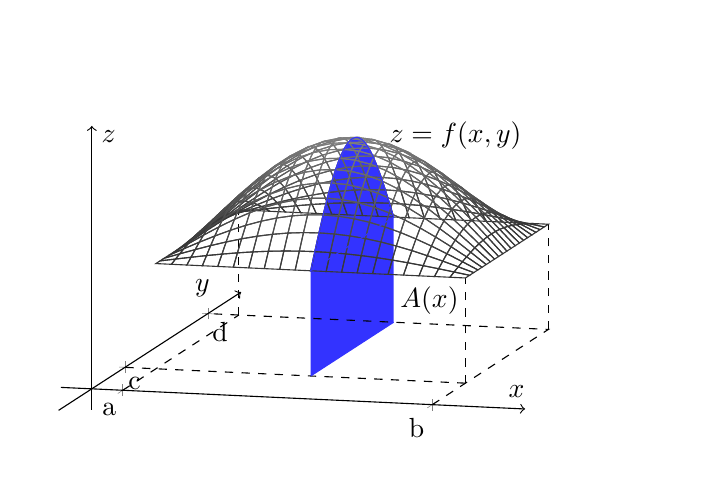
\begin{tikzpicture}[baseline]
\begin{axis}[
axis lines = middle,
unit vector ratio*=3 3 1,
scale=1.6, xmin=-0.1, xmax=1.4, ymin=-0.4, ymax=1.8, zmin = -0.2, zmax = 2.5,
view={15}{10},
%grid = major,
xtick={0.1, 1.1},
ytick={0.4, 1.4},
ztick = {0},
xticklabels = {a, b},
yticklabels = {c, d},
zticklabels = {}, 
xlabel=$x$,
ylabel=$y$,
zlabel = $z$,
axis line style = {->},
]
%\addplot[name path=up,samples=100,domain=0:pi]({cos(deg(x))+1.2},{sin(deg(x))+1.2});
%\addplot[name path=line1,domain=0.4:0.4,y domain=-0.2:1.2]{1};
%\addplot[name path=xaxis,domain=0:2]{0};
%\draw[thick](axis cs:1,0) -- (axis cs:1,3);
%\addplot[gray!30]fill between[of=curve and xaxis,soft clip={domain=1:2}];
\coordinate (A) at (0.1,0,0);
\coordinate (B) at (1.1,0,0);
\coordinate (C) at (0,1.4,0);
\coordinate (D) at (1.1,1.4,0);
\coordinate (E) at (axis cs:0.1,1.4,0);
\coordinate (F) at (axis cs:1.1,0.4,1);
\coordinate (G) at (axis cs:0.1,1.4,1);
\coordinate (H) at (axis cs:1.1,1.4,1);
\coordinate (I) at (1.1,0.4,0);
\coordinate (J) at (0,0.4,0);
\draw[thin,dashed] (B) -- (D) -- (C);
\draw[thin,dashed] (I) -- (F);
\draw[thin,dashed] (E) -- (G);
\draw[thin,dashed] (D) -- (H);
\draw[thin,dashed] (A) -- (E);
\draw[thin,dashed] (I) -- (J);
%\draw[thick,densely dashed] (B) -- (C);
%\draw[thick,densely dashed] (D) -- (B);
%\draw[thick] (A) -- (B) -- (D) -- (C) -- cycle;

%\addplot3[surf,shader=flat,colormap={blackwhite}{color=(black!50) color=(black!20)},samples=50,domain=0:1, y domain=0:1,]{1+sin(deg(pi*x))*sin(deg(pi*y))};
\addplot3[mesh,colormap={blackwhite}{color=(black!80) color=(black!50)},samples=21,domain=0.1:1.1, y domain=0.4:1.4,]{1+sin(deg(pi*(x-0.1)))*sin(deg(pi*(y-0.4)))};

\node at (axis cs:0.8,1.4,1.8) {$z=f(x,y)$};
%\draw[thick,fill=green!30](axis cs:0.6,0,0) -- (axis cs:0.6,1,0) -- (axis cs:0.6,1,2.2) -- (axis cs:0.6,0,2.2) --cycle;
%\addplot3[blue]fill between[of=A and B];
%\draw[thick](axis cs:0.6,0,0) -- (axis cs:0.6,1,0) -- (axis cs:0.6,1,2.2) -- (axis cs:0.6,0,2.2) --cycle;
\addplot3[name path=A,domain=0.4:1.4,color=blue!80]({0.6},{x},{1+sin(deg(0.5*pi))*sin(deg(pi*(x-0.4)))});
\addplot3[name path=B,domain=0.4:1.4,color=blue!80]({0.6},{x},{0});
\addplot3[blue!80]fill between[of=A and B];
\node at (axis cs:0.85,0.9,0.5) {$A(x)$};
%\addplot3[surf,y domain=-0.2:1.2]{0.4};
\end{axis}
%\begin{axis}
%\addplot3[surf,shader=flat]coordinates{
%(0.4,-0.2,-0.2) (0.4,1.2,-0.2) (0.4,1.2,2.2) (0.4,-0.2,2.2) (0.4,-0.2,-0.2)};
%\end{axis}
\end{tikzpicture}

\end{document}